\begin{figure}
\tikzstyle{arrow} = [thick,->,>=stealth]
\tikzstyle{arrowd} = [thick,dashed,->,>=stealth]
\centering
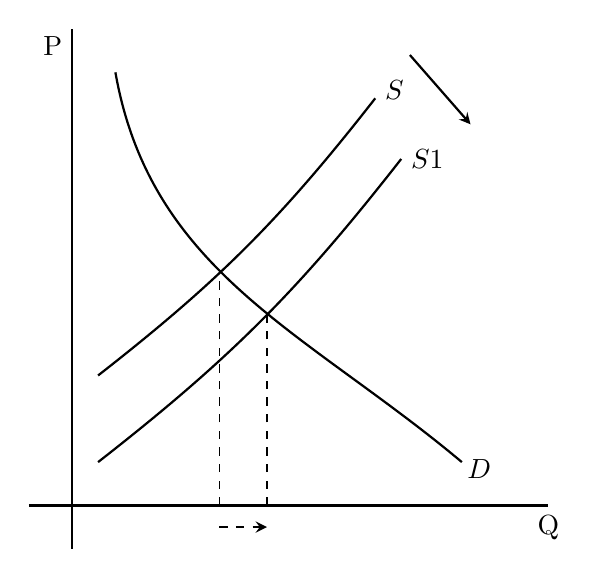
\begin{tikzpicture}[scale=1.1]

% Axis
\draw [thick] (-0.5,-0.0) --(5.5,0);
\draw [thick] (0,-0.5) -- (0,5.5);
\node [left] at (0,5.3) {P};
\node [below] at (5.5,0) {Q};

%Downward slopping line
\draw [thick] (0.5,5) to [out=280,in=140] (4.5,0.5);
\node [above] at (4.7,0.2) {$D$};

% Upward Slopping S1
\draw [thick] (0.3,0.5) to [out=38,in=232] (3.8,4);
\node [right] at (3.8,4) {$S1$};

% Upward Slopping S
\draw [thick] (0.3,1.5) to [out=38,in=232] (3.5,4.7);
\node [right] at (3.5,4.8) {$S$};

% dashed lines
\draw [dashed](1.7,0)--(1.7,2.7);
\draw [dashed](2.25,0)--(2.25,2.3);

\draw [arrow] (3.9,5.2) -- (4.6,4.4);
\draw [arrowd] (1.7,-0.25) -- (2.25,-0.25);

\end{tikzpicture}
  \caption{Benefits of Cheaper Transport}
  \label{fig:cheaper_transport}
\end{figure}
